\subsection{静态背景和动态物体的同时重建}
\label{subsec:static_and_dynamic}

尽管动态物体对于相机位姿的求解会造成干扰,但在某些应用情形而言,动态物体的三维信息也是我们感兴趣的部分。在这种情形下,算法就需要完成静态背景与动态物体的同时重建。一般而言该类方法会更为复杂与困难。算法除了要通过识别静态背景以获得良好的位姿信息,还需对于每一个运动物体都维护独立的坐标系和地图以进行相应的配准和融合。

对于静态背景和动态物体的同时重建问题,其核心过程可分为两大部分:静态与动态的分割,以及每一部分的数据融合。良好的分割结果可提升相机位姿的求解精度,从而使得重建结果的准确度提升;而对于不同动态物体使用合适的融合方式则影响了所关注物体重建的结果。

目前,对于动态物体与静态场景的分割问题,研究者往往使用RGBD传感器作为算法的输入,以获得更为优良准确的单帧三维信息。Zhang和Xu~\cite{2017MixedFusion}维护了每一个时刻的场景模型(Scene Model),以对输入的每一帧深度信息进行初步配准,区分出静态部分和动态物体。场景的静态部分用于相机位姿的估计,而对于动态的部分作者则参考了Newcombe提出的DynamicFusion~\cite{2015DynamicFusion},使用了一种基于图节点的运动表示结构(Graph Node-based Motion Representation)来进行动态物体的融合,以完成对非刚性运动物体(如人体、窗帘等)的模型融合。不过,由于算法本身对于动态物体采用的是DynamicFusion的融合框架,该方法只用到了输入的深度信息而丢弃了RGB图像信息,并且难以处理动态物体发生拓扑变化的情况。Caccamo等人~\cite{2017Joint3D}使用了自底向上的特征分类的方式进行物体的识别与分割。算法维护了一个静态的地图,并对于输入的每一帧进行特征计算与配准。根据配准之后的误差,将误差较高的部分聚合分离出来,从而判断出与相机运动不一致的动态物体,并维护该动态物体的地图,完成融合。该算法假设场景中只有一个刚性运动的物体,使用场景较为受限。

\begin{figure}[htbp]
	\centering
	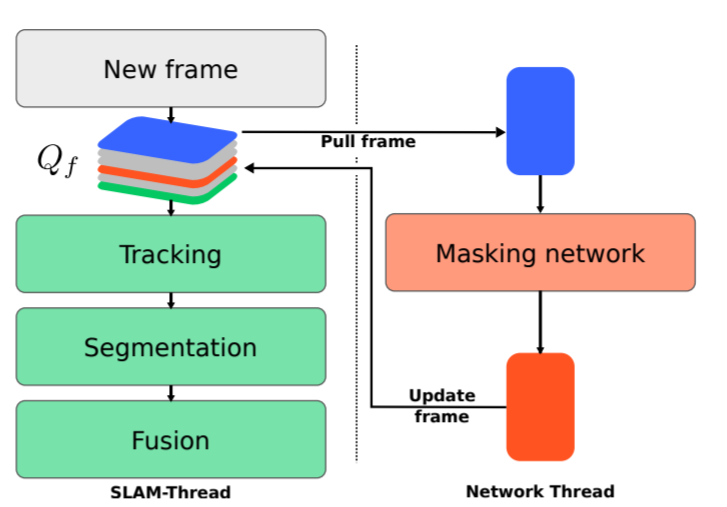
\includegraphics[width=0.9\textwidth]{figs/2-2/maskfusion.png} 
	\label{fig:MaskFusion-framework}
	\caption{MaskFusion算法结构框图。}
\end{figure}

对于多个物体的跟踪与重建,R\"unz和Agapito~\cite{2017CoFusion}提出了Co-Fusion,用于处理多个不同物体的运动。该方法通过运动和语义信息将物体从场景中分割出来,然后对这些物体分别进行跟踪和重建。算法分割出物体后,可对每一部分的三维数据分别进行基于面元的数据融合,以处理不同物体的刚体运动,获得它们的三维模型。这种基于物体分割的动态物体重建会更适用于机器人相关的应用。算法可以对运动的物体获得较为准确的三维信息,从而使得机器人可以与环境进行更为丰富的交互。R\"unz等人之后基于深度学习的方法提出了MaskFusion~\cite{2018MaskFusion},算法将Mask-RCNN~\cite{2017MaskRCNN}的分割结果与形状信息相结合,替代了原有的分割模块,从而在物体的分割边缘上能得到更好的表现,如图~\ref{fig:MaskFusion-framework}所示。该类方法将语义信息与物体形状相结合,从而获得更加完善的室内场景的物体分割结果。但从另一个角度来说,物体的语义信息依赖于模型的训练集。实验过程中的运动物体需要在训练集中出现过才能得到合理的分割结果,这也是使用语义作为分割标准的一个无法避免的弊端。

相较于使用语义信息进行自顶向下的分割,Xu等人 ~\cite{2019MIDFusion}使用几何和运动信息进行场景物体的分割。对于分割后的物体,算法分别对这些物体进行物体姿态的估计、建图以及融合。该方法对于每个物体都维护了一个基于体素的子图(Object-level dynamic volumetric map),从而相应的定位和融合算法可以在物体层面上增量的进行。

总体而言,动态物体与静态场景的同时重建问题是一个较为困难的问题,即便输入为信息最为丰富的RGBD数据,目前也很难给出一个普适性的解决方案,均需要根据情况增加约束以使得问题可解。研究大多着眼于如何将静态与动态部分分割开,并使用适当的模型来描述动态物体的运动。尽管目前对于单一物体的简单运动可以恢复出较好的模型,但对于多物体复杂运动,考虑到相应的运算开销,常常难以获得较为鲁棒、准确的结果。
